\documentclass[main.tex]{subfiles}

\begin{document}

\subsection{Secondo esercizio}

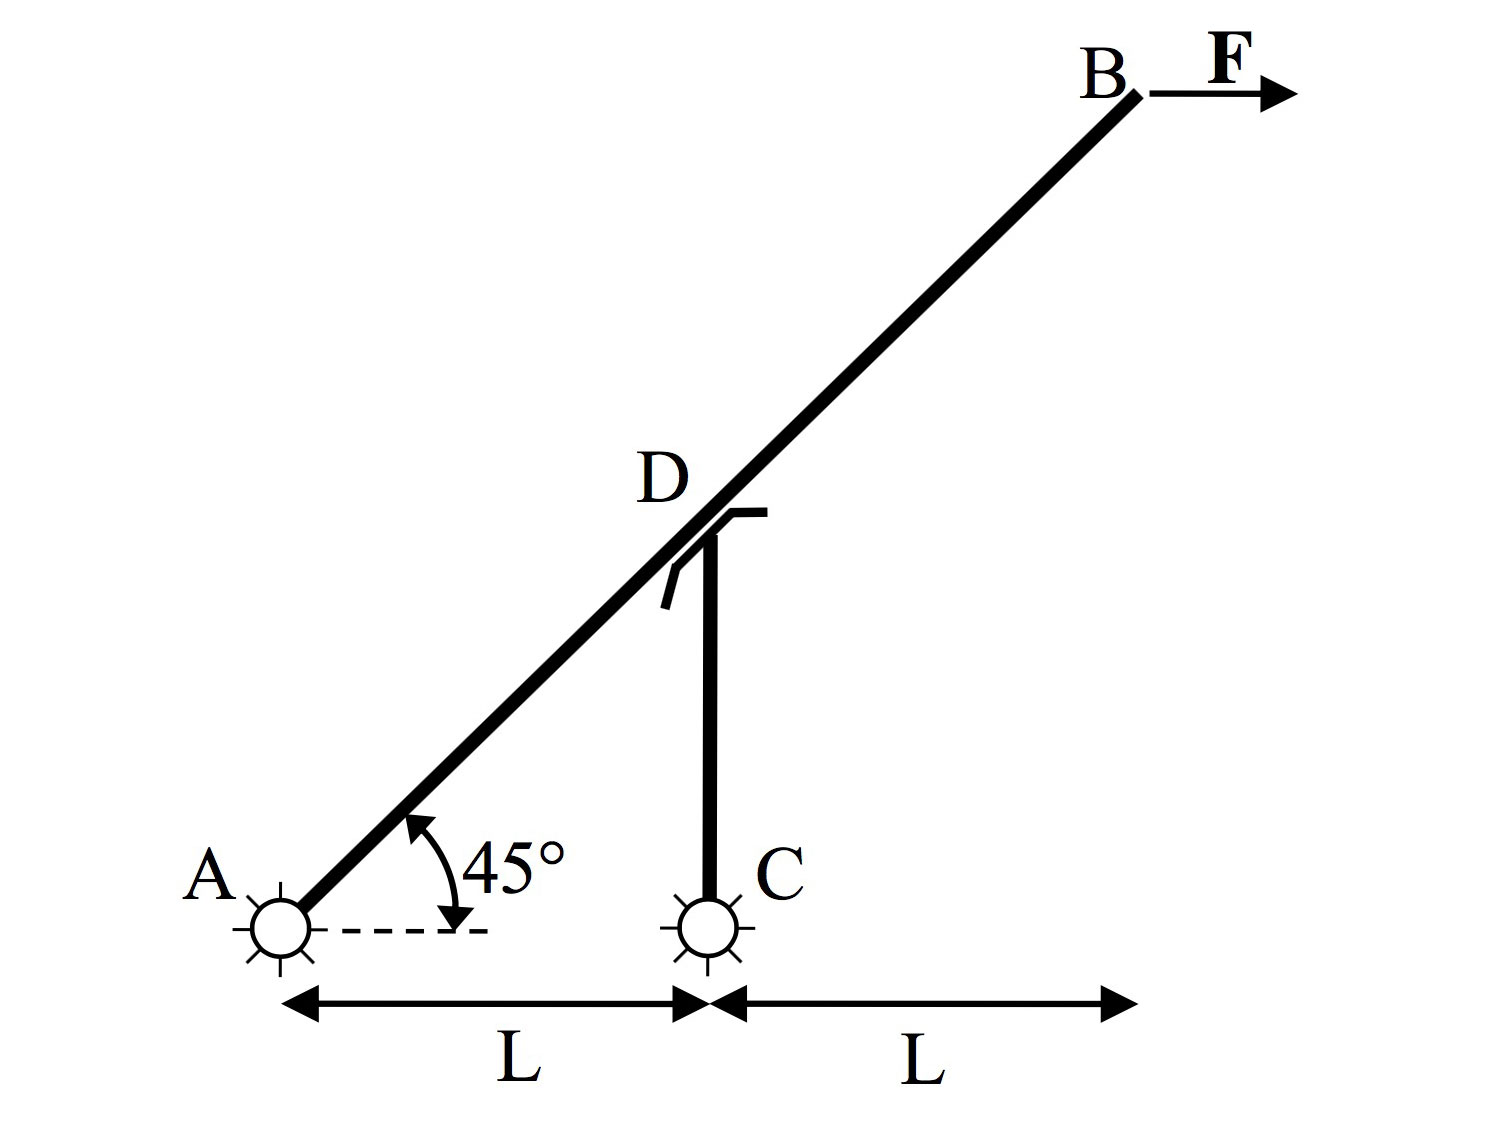
\includegraphics[width=\textwidth]{2014-2409-2.jpg}

La struttura in figura è soggetta alla sola forza orizzontale F.

Si chiede di calcolare:

\begin{enumerate}
\item Le reazioni vincolari in A e C.
\item Le azioni interne nell’asta AB (disegnare i corrispondenti diagrammi).
\end{enumerate}

\clearpage

\subsection{Soluzione secondo esercizio}

\subsubsection{Osservazioni}

\begin{enumerate}
\item La struttura è composta da 2 corpi rigidi, le aste, e 3 vincoli doppi: due cerniere e un pattino.
\item Il pattino ha una reazione assiale che agisce tangenzialmente sull'asta, ad un angolo di $45\deg$.
\end{enumerate}

\subsubsection{Analisi preliminare di isostaticità}
Verifico che $gdl_{tot} = gdv_{tot}$:
\begin{figure}[H]
  \begin{subfigure}[b]{.5\textwidth}
  \centering
  \[
  	gdv: \begin{cases}
		gdv_{cerniera_{esterna}} = 4\\
		gdv_{pattino} = 2
  	\end{cases}
  \]
  \caption{Gradi di vincolo del sistema.}
  \end{subfigure}
  \hfill
  \begin{subfigure}[b]{.5\textwidth}
  \centering
  \[
  	gdl: \begin{cases}
  		gdl_{aste} = 6\\
  	\end{cases}
  \]
  \caption{Gradi di libertà del sistema.}
  \end{subfigure}
  \caption{Verifica preliminare di isostaticità.}
\end{figure}

\subsubsection{Primo punto}

\paragraph{Vincoli esterni}
Per prima cosa descriviamo con un sistema di equazioni di equilibrio statico le reazioni vincolari esterne sotto l'effetto della forza F, rappresentate in figura \ref{vincoli_esterni_2014_2409_2}:
\\

Scelgo arbitrariamente come punto in cui calcolare il momento totale A, normalmente si sceglie il punto con più forze applicate o dove è già applicato un momento (per esempio un incastro) per semplificare i calcoli.
\\

Per definire il segno di un momento, guardo la direzione di rotazione verso cui la forza spinge il vettore di spostamento normale. Si sceglie una direzione positiva arbitrariamente, basta mantenerla per l'intera equazione, per esempio in questo esercizio scelgo positiva la direzione oraria.

\begin{enumerate}
\item Il vettore $\vec{F}$ ha un vettore di spostamento normale di modulo $2L$ e ruota in senso \textbf{orario}.
\item Il vettore $\vec{H}_C$ ha un vettore di spostamento normale di modulo $L$ e ruota in senso \textbf{anti-orario}.
\item Il vettore $\vec{V}_C$ ha un vettore di spostamento unicamente tangente, per cui non impone momento.
\end{enumerate}

\[
\begin{cases}
	H_A + H_C = F	\\
	V_A - V_C = 0\\
	M_A = 0 = 2LF + -LV_C
\end{cases}
\Longrightarrow
\begin{cases}
	H_A + H_C = F	\\
	V_A = 2F\\
	V_C = 2F
\end{cases}
\]

\begin{figure}[H]
\centering
\resizebox{.5\textwidth}{!}{% First image 2015 06 29

\begin{tikzpicture}

  \tiny


  \point{c}{0}{0}
  \point{c1}{0}{0.8}
  \point{c2}{-0.8}{0}
  \point{a}{2-1.41421}{1.41421}
  \point{a1}{2-1.41421}{0.8+1.41421}
  \point{d}{2}{0}
  \point{b}{2+1.41421}{-1.41421}
  \point{b1}{2+1.41421}{-1.41421-1.3}

  \beam{2}{c}{d}[0][1];
  \beam{2}{a}{b};

  \load{1}{a}[180][0.5]
  \load{1}{a1}[270][0.5]

  \load{2}{c}
  \load{1}{c}[180][0.5]
  \load{1}{c}[270][0.5]

  \load{1}{b1}[90][1]

  \notation{1}{c}{$\vec{M}_C$}[below right]
  \notation{1}{c}{$\vec{H}_C$}[below left]
  \notation{1}{c}{$\vec{V}_C$}[above right]

  \notation{1}{a}{$\vec{H}_A$}[below left]
  \notation{1}{a}{$\vec{V}_A$}[above right]

  \notation{1}{b}{$\vec{F}$}[below right]

  % \notation{1}{a1}{$\vec{H}_A$}
  % % \notation{1}{d1}{$\vec{R}_D$}
  % % \notation{1}{b1}{$\vec{H}_B$}[below left]
  % \notation{1}{c1}{$\vec{F}$}[above left]

  %  % \support{3}{o};

  %  % %Degrees
  %  % \notation{1}{o}{$\alpha$}[above];
  %  % \notation{1}{a}{$\beta$}[above];

  %  % \notation{5}{o}{a}[$a$];
  %  % \notation{5}{a}{b}[$b$];
  %  % \notation{5}{o}{b}[$c$];

\end{tikzpicture}}
\caption{Analisi dei vincoli esterni}
\label{vincoli_esterni_2014_2409_2}
\end{figure}

\paragraph{Asta CD}
Questa asta è posta tra un pattino ed una cerniera. Le reazioni della cerniera devono quindi coincidere con le componenti della reazione assiale del pattino.
\\

Il pattino è posto in un modo per cui la sua reazione assiale è a $45\deg$, per cui le componenti $R_{x_D}=R_{y_D}$.

\begin{center}
\framebox[4in]{
\begin{minipage}[t]{3.5in}
{\Large{\danger}} \textbf{N.B.}
La direzione del momento legato alla reazione del vincolo \textbf{pattino}, come negli altri vincoli del resto, è legata alla direzione della forza tangente. Se la forza tangente è orientata verso il basso (in questo caso la reazione assiale) il momento è orientato in senso \textbf{anti-orario}, altrimenti è orientato in senso \textbf{orario} quando la reazione tangente è verso l'alto.
\end{minipage}}
\end{center}

\begin{figure}[H]
\centering
\resizebox{.3\textwidth}{!}{% First image 2015 06 29

\begin{tikzpicture}

  \tiny

  \point{a}{0}{0}
  \point{c}{1}{0}
  \point{b}{2}{2}
  \point{d}{1}{1}

  % \beam{2}{a}{b}
  \beam{2}{c}{d}

  % \load{1}{b}[180][0.5]
  % \load{1}{a}[0][0.5]
  % \load{1}{a}[90][0.5]
  \load{1}{c}[0][0.5]
  \load{1}{c}[270][0.5]

  \load{1}{d}[180][0.5]
  \load{1}{d}[90][0.5]
  \load{3}{d}

  \notation{1}{d}{$\vec{R}_{y_D}$}[above right]
  \notation{1}{d}{$\vec{R}_{x_D}$}[above left]

  \notation{1}{c}{$\vec{V}_C$}[below left]
  \notation{1}{c}{$\vec{H}_C$}[above right]

\end{tikzpicture}}
\caption{Analisi delle reazioni vincolari nell'asta CD}
\label{asta_CD_2014_2409_2}
\end{figure}

\[
	\begin{cases}
		H_C = R_{x_D}\\
		V_C = R_{y_D}\\
		M_D = LH_C\\
		R_{y_D} = R_{x_D}
	\end{cases}
	\Longrightarrow
	\begin{cases}
		H_C = 2F
		M_D = L2F
	\end{cases}
\]

Ora posso quindi risolvere il sistema precedente che risulta:

\[
\begin{cases}
	H_A = -F	\\
	H_C = 2F\\
	V_A = 2F\\
	V_C = 2F
\end{cases}
\]

\subsubsection{Riassunto soluzione primo punto} Mantenendo il verso dei vettori coerente con quello in figura \ref{vincoli_esterni_2014_2409_2}, le reazioni vincolari sono:
\begin{figure}[H]
  \begin{subfigure}[b]{.5\textwidth}
  \centering
  \[
  	A: \begin{cases}
		H_A = -F\\
		V_A = 2F
  	\end{cases}
  \]
  \caption{Reazioni vincolari in A.}
  \end{subfigure}
  \hfill
  \begin{subfigure}[b]{.5\textwidth}
  \centering
  \[
  	C: \begin{cases}
  		V_C = 2F\\
  		H_C = 2F
  	\end{cases}
  \]
  \caption{Reazioni vincolari in C.}
  \end{subfigure}
\end{figure}

\subsubsection{Secondo punto}

\begin{figure}[H]
\centering
\resizebox{.3\textwidth}{!}{\input{chapters/2/2014/2409/2/asta_ab.tex}}
\caption{Reazioni vincolari nell'asta AB}
\label{asta_AB_2014_2409_2}
\end{figure}

Proiettando i vettori sugli assi normali e tangenti all'asta, ottengo:

\[
A: \begin{cases}
	T = \sqrt{2}F + \dfrac{\sqrt{2}}{2}F = \dfrac{3\sqrt{2}}{2}F \\
	N = \sqrt{2}F - \dfrac{\sqrt{2}}{2}F = \dfrac{\sqrt{2}}{2}F\\
\end{cases}
\]

\[
D: \begin{cases}
	T = \sqrt{2}F + \sqrt{2}F = 2\sqrt{2}F \\
	N = \sqrt{2}F - \sqrt{2}F = 0\\
\end{cases}
\]

\[
F: \begin{cases}
	T = \dfrac{\sqrt{2}}{2}F\\
	N = \dfrac{\sqrt{2}}{2}F
\end{cases}
\]

\paragraph{Sforzo normale}
Lo sforzo normale impone una trazione, per cui è per convenzione positivo:

\begin{figure}[H]
\centering
\resizebox{.3\textwidth}{!}{% First image 2015 06 29

\begin{tikzpicture}

  \tiny


  \point{c}{0}{0}
  \point{a}{0}{1}
  \point{b}{1}{0}
  \point{d}{2}{0}

   \beam{2}{c}{d}[0][1];

  \internalforces{c}{b}{1}{1}[0][blue];

\end{tikzpicture}}
\caption{Sforzo normale nell'asta AB}
\end{figure}

\paragraph{Taglio}
Il taglio nella parte inferiore dell'asta impone una rotazione \textbf{anti-oraria} ed è pertanto negativo. Nella parte superiore, invece, impone una rotazione oraria e quindi è \textbf{positivo}.

\begin{figure}[H]
\centering
\resizebox{.3\textwidth}{!}{% First image 2015 06 29

\begin{tikzpicture}

  \tiny


  \point{c}{0}{0}
  \point{c1}{0}{0.8}
  \point{c2}{-0.8}{0}
  \point{a}{2-1.41421}{1.41421}
  \point{a1}{2-1.41421}{0.8+1.41421}
  \point{d}{2}{0}
  \point{d1}{2-0.8}{0}
  \point{b}{2+1.41421}{-1.41421}
  \point{b1}{2+1.41421}{-1.41421-1.3}

  \beam{2}{a}{b};

  \internalforces{a}{d}{-0.707}{-0.707}[0][blue];
  \internalforces{d}{b}{0.707}{0.707}[0][red];

\end{tikzpicture}}
\caption{Taglio nell'asta AB}
\end{figure}

\paragraph{Momento flettente}
Per determinare il lato delle \textbf{fibre tese} osserviamo il vettore $T_A$ (o analogamente $T_F$). Questo vettore flette le fibre del lato destro, che quindi saranno identificate come fibre tese.

Il momento flettente, partendo dall'estremo A, aumenta linearmente raggiungendo il massimo nel punto di discontinuità D, in cui assume il valore di $M_{A_{max}} = \dfrac{2}{\sqrt{2}}L \dfrac{3\sqrt{2}}{2}F = 3LF$.
\\
Procedendo invece dall'estremo B, aumenta sempre linearmente raggiungendo il massimo in D, ma qui assume il valore $M_{B_{max}} = \dfrac{2}{\sqrt{2}}L \dfrac{\sqrt{2}}{2}F = LF$.

\begin{figure}[H]
\centering
\resizebox{.3\textwidth}{!}{% First image 2015 06 29

\begin{tikzpicture}

  \tiny


  \point{c}{0}{0}
  \point{c1}{0}{0.8}
  \point{c2}{-0.8}{0}
  \point{a}{2-1.41421}{1.41421}
  \point{a1}{2-1.41421}{0.8+1.41421}
  \point{d}{2}{0}
  \point{d1}{2-0.8}{0}
  \point{b}{2+1.41421}{-1.41421}
  \point{b1}{2+1.41421}{-1.41421-1.3}

  \beam{2}{a}{b};

  \internalforces{a}{d}{0}{-0.707}[0][red];
  \internalforces{d}{b}{-0.707}{0}[0][red];

\end{tikzpicture}}
\caption{Momento flettente nell'asta AB}
\end{figure}

\end{document}
